\documentclass[tikz, border=10pt]{standalone}
\usetikzlibrary{external}
\tikzexternalize


\begin{document}
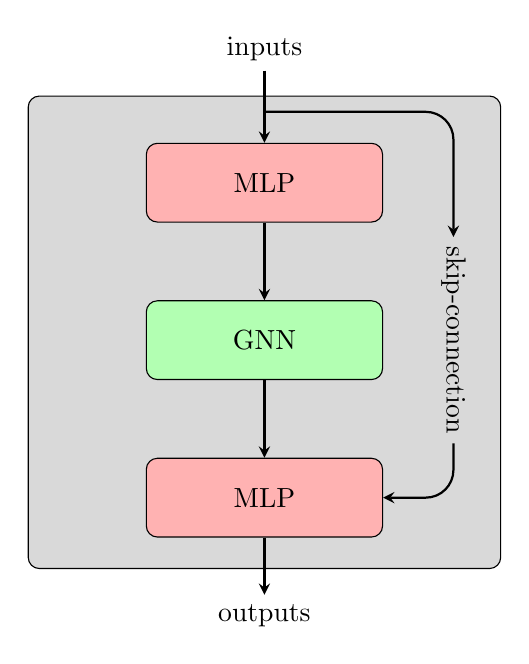
\begin{tikzpicture}
\tikzstyle{MLP} = [rectangle, rounded corners, minimum width=3cm, minimum height=1cm,text centered, draw=black, fill=red!30]
\tikzstyle{GNN} = [rectangle, rounded corners, minimum width=3cm, minimum height=1cm,text centered, draw=black, fill=green!30]
\tikzstyle{IN} = [rectangle, rounded corners, minimum width=6cm, minimum height=6cm,text centered, draw=black, fill=gray!30]

\tikzstyle{arrow} = [thick, rounded corners=10pt, ->,>=stealth]
\tikzstyle{line} = [thick,-,>=stealth]

    % Your TikZ code here

	\node (in) at (0, -1.9) [IN] {};
	
    \node (start) [MLP] {MLP};
    \node (gnn) at (0, -2) [GNN] {GNN};
    \node (end) at (0, -4) [MLP] {MLP};
    
    \node (input) at (0, 1.7) {inputs};
    \node (output) at (0, -5.5) {outputs};
    
    \node (skip) at (2.4, -2) {\rotatebox{-90}{skip-connection}};
    
    \draw [arrow] (input) -- (start);
    \draw [arrow] (start) -- (gnn);
    \draw [arrow] (gnn) -- (end);
    
	\draw [arrow] (0, 0.9) -| (skip);
    
    \draw [arrow] (skip) |- (end);
    \draw [arrow] (end) -- (output);
\end{tikzpicture}
\end{document}